%% LyX 2.0.3 created this file.  For more info, see http://www.lyx.org/.
%% Do not edit unless you really know what you are doing.
\documentclass[english]{article}
\usepackage[T1]{fontenc}
\usepackage[latin9]{inputenc}
\usepackage{geometry}
\usepackage{amsmath}
\usepackage{graphicx}
\usepackage{paralist}
\geometry{verbose,tmargin=0.75in,bmargin=0.75in,lmargin=0.75in,rmargin=1in}


\makeatletter

%%%%%%%%%%%%%%%%%%%%%%%%%%%%%% LyX specific LaTeX commands.
%% Because html converters don't know tabularnewline
\providecommand{\tabularnewline}{\\}

\makeatother

\usepackage{babel}
\begin{document}
\thispagestyle{empty}

\begin{tabular*}{1\textwidth}{@{\extracolsep{\fill}}lr}
\textbf{ID:} 03 & \textbf{Collaborator \#1:} Chen, Josh\tabularnewline
\textbf{Name:} Al-Naji, Nader & \textbf{Collaborator \#2:} Last Name, First Name\tabularnewline
\hline 
\end{tabular*}

\medskip{}


\begin{center}
\begin{Large}\textbf{Solution to HW 6, Problem 1}\end{Large}
\par\end{center}

\begin{center}
\begin{large}\textbf{COS 340 - Spring 2012}\end{large}
\par\end{center}

\bigskip{}


% Begin sol%
This is a variation of the Weighted-Majority algorithm for the experts problem:
\newline\newline
1. Each expert begins with a weight of $1$ (as before).\newline
2. We predict based on a weighted majority vote of the experts (as before).\newline
3. If an expert makes a mistake, we penalize him by dividing the weight by 2, \textbf{but only if
the weight was at least 1/4 of the average weight of the experts at that time} (this is new).
\newline
\newline
\textbf{1. Prove that at any time during the execution of this algorithm, the weight of any expert is at least 1/8 of the
average weight of the experts at that time.}
\newline
\newline
We can show this using strong induction on the time step of the algorithm. Let $Q(s)$ be the following statement:
\newline
\newline
$Q(s) =$ ``At time step s, the weight of any expert is at least the 1/8 of the average weight of the experts at that time.''
\newline\newline
\textbf{Base: $s = 1$:}
\newline
Let $w_1^{(1)}, ..., w_n^{(1)}$ be the weights of each of the $n$ experts at time step $1$. Also let $W$ be the total weight
of all the experts, ie $W = \sum\limits_{i=1}^{n} w_i$. This makes the average weight $W_{ave} = W/n = n/n = 1$ for the first time step.
At the first time step, $w_i = 1 \mbox{ } \forall \mbox{ } i \in \{1, ..., n\} \rightarrow w_i = W_{ave} > (1/8)W_{ave} \mbox{ } \forall \mbox{ } i \in \{1, ..., n\}$.
So the statement holds for $s = 1$.
\newline
\newline
\textbf{Step: Assume $Q(s)$ holds for all $s \in {1, ..., t}$ and show it holds for $s = t+1$:}
\newline
If $Q(s)$ holds for time step $t$ then at time step $t$, we must have $w_i^{(t)} \geq (1/8)W_{ave} \mbox{ } \forall \mbox{ } i \in \{1, ..., n\}$. Now to get to
$s = t+1$, we must run the algorithm on all the experts at this time step and make sure that the statement holds for $t+1$. For any expert $w_i$, one of three things
can happen so we will check these three cases for any expert $i$ with weight $w_i$ to make sure that the statement is not violated:
\newline\newline
1. $w_i^{(t)} < (1/4) W_{ave}$:
\newline
If this happens, regardless of whether or not expert $i$ is right or wrong, his weight will remain unchanged and so, because we had that
 $w_i^{(t)} \geq (1/8)W_{ave} \mbox{ } \forall \mbox{ } i \in \{1, ..., n\}$ at time step $t$, we will have $w_i^{(t+1)} = w_i^{(t)} \geq (1/8)W_{ave}$ and
 the statement will hold for $t+1$ for 
 this expert. Note that this is true since $W_{ave}$ can never increase between iterations and therefore if the weight of an expert remains the same, the quantity
 $w_i - W_{ave}$ can only increase at each iteration.
\newline\newline
2. $w_i \geq (1/4)W_{ave}$ and expert $i$ is correct.
\newline
If this happens, we don't change expert $i$'s weight and so the statement will hold because $w_i^{(t+1)} = w_i^{(t)} \geq (1/4)W_{ave}\geq (1/8)W_{ave}$
for this expert. Again, note that this is true since $W_{ave}$ can never increase between iterations and therefore if the weight of an expert remains the same, the quantity
 $w_i - W_{ave}$ can only increase at each iteration.
\newline
\newline
3. $w_i \geq (1/4)W_{ave}$ and expert $i$ is wrong.
\newline
If this happens, the algorithm dictates that we must divide expert $i$'s weight in half. However, this doesn't violate the statement because expert
$i$'s weight will always be greater than $1/8W_{ave}$ after division. Showing this: $w_i^{(t+1)} = w_i^{(t)}/2 \geq (1/2)(1/4)W_{ave} = (1/8) W_{ave}$.
And since $W_{ave}^{t+1} \leq W_{ave}^t$, this will hold at the end of the iteration as well.
\newline
\newline
Thus, having shown that the statement is true for the base and the step, we conclude that it must be true for all $t$.
\newline
\newline
\textbf{2. Consider a step when the algorithm makes a mistake. Let $\phi$ be the sum of weights of experts before this step and let $\phi'$ be the sum of
the weights after this. Prove that $\phi' \leq (7/8) \phi$.}
\newline
\newline
Let $L$ be the set of incorrect experts at the beginning of the time step with weight $w_i < (1/4) W_{ave}/n = (1/4)\phi/n$ and 
$H$ be the set of incorrect experts at the beginning of the time step with weight $w_i \geq (1/4)W_{ave} = (1/4)\phi /n$. Let $W_L = \sum\limits_{i \in L}^{} w_i$ and $W_H = \sum\limits_{i \in H}^{} w_i$ be the sum of the weights of the incorrect experts in each group. Because each incorrect expert in $L$ contributes at most $(1/4)\phi /n$, 
we know that $W_L \leq (1/4) \phi$ because no more than $n$ experts can be in this group. We also have the following relation for the total weight: $W_{bad} = W_L + W_H \geq \phi /2$
because we know that the algorithm made a mistake and because $L$ and $H$ are disjoint and cover the set of incorrect experts. Thus, using this final relation, we can solve
for $W_H$ and get: $W_L + W_H \geq \phi /2 \rightarrow W_H \geq \phi / 2 - W_L \rightarrow W_H \geq \phi / 2 - \phi/4 \rightarrow W_H \geq \phi / 4$. Because every expert in $H$
has a weight $w_i \geq (1/4)W_{ave}$, the algorithm dictates that their weight will be cut in half. Thus, at each iteration, after making a mistake, the experts will lose
an amount of weight equal to $W_{lost} = W_H/2 \geq \phi / 8$, which implies that the total weight after each incorrect prediction cannot be more than $\phi - \phi /8 = (7/8)\phi$.
Thus, $\phi' \geq (7/8)\phi$.
\newline
\newline
\textbf{Prove that in any interval of time $[t_1, t_2]$, the number of mistakes made by the algorithm is at most $O(m + \log n)$ where $m$ is the number of mistakes
made by the best expert in that interval and $n$ is the total number of experts.}
\newline
\newline
Let $\phi_1$ be the total weight at time $t_1$ and let $\phi_2$ be the total weight at time $t_2$. Let $M$ be the number of mistakes made by the algorithm during the
interval and let $m$ be the number of mistakes made by the best expert during the interval. In the interval, the algorithm loses at least $(1/8)$ of its weight for every
incorrect prediction. So we have as an upper bound on $\phi_2$: $\phi_2 \leq (7/8)^M \phi_1$. As a lower bound, $\phi_2$ cannot be lower than the weight of the best expert at any time. 
Since the best expert starts with weight $w_i \geq (1/8)\phi / n$ at time $t_1$ by construction and since the best expert loses at most $1/2$ of his weight for 
every incorrect prediction, we have a lower bound on the weight at time $t_2$: $\phi_2 \geq (1/2)^m (1/8)\phi_1/n$. This gives us the following equation:
\newline
\newline
$(1/2)^m (1/8)\phi_1/n \leq \phi_2 \leq (7/8)^M \phi_1 \rightarrow (1/2)^m (1/(8n))\phi_1 \leq (7/8)^M \phi_1
\newline\rightarrow (2)^m 8n \geq (8/7)^M \rightarrow (8/7)^M \leq (2)^m 8n \rightarrow M \log(8/7) \leq m + \log(n) + \log(8) \rightarrow M \leq c1 (m + \log n)
\newline\rightarrow M = O(m + \log n)$ by the definition of big-O.

% End sol%

\pagebreak{}

\thispagestyle{empty}

\begin{tabular*}{1\textwidth}{@{\extracolsep{\fill}}lr}
\textbf{ID:} 03 & \textbf{Collaborator \#1:} Chen, Josh\tabularnewline
\textbf{Name:} Al-Naji, Nader & \textbf{Collaborator \#2:} Last Name, First Name\tabularnewline
\hline 
\end{tabular*}

\medskip{}


\begin{center}
\begin{Large}\textbf{Solution to HW 6, Problem 2}\end{Large}
\par\end{center}

\begin{center}
\begin{large}\textbf{COS 340 - Spring 2012}\end{large}
\par\end{center}

\bigskip{}


% Begin sol%
Recall in class and in the notes we saw that for any $\epsilon$ on can give am experts algorithm in which the expected number of mistakes $E[M]$
is bounded by $\frac{m}{1 - \epsilon} + \frac{\ln n}{\epsilon}$ where $m$ is the number of mistakes the best expert makes. The aim of this exercise
is to show that this performance cannot be improved by much. For simplicity, we will show that:
\begin{center}
\large $E[M] \leq \frac{m}{1-\epsilon} + \frac{\ln n}{\epsilon^{1/2}}$
\end{center}
is impossible to attain. Let's fix $n = 2$. In other words, there are only two experts. Denote the number of prediction steps performed by $T$.
Suppose that the outcomes $o_1, ..., o_T$ we are trying to predict are just independent fair coin tosses distributed as $Bern(1/2)$. Suppose further
that the ``experts'' are also just giving random advice given by fair coin tosses, independently of the actual outcomes or of each other. Denote
the sequence of ``advice'' given by the first expert by $a_1, ..., n_T$ and the ``advice'' given by the second expert by $b_1, ..., b_T$. Note that
since the advice is independent of the outcomes and the outcomes are fair coin tosses, the best prediction strategy (and in fact any prediction
strategy) will satisfy:
\begin{center}
$E[M] = T/2$
\end{center}
1. Out first goal is to estimate $m$- the number of mistakes made by the more successful of the two experts. Note that here $m$ is also a random
variable. Our goal will be to show that:
\begin{center}
$E[m] < T/2 - \Omega(\sqrt{T})$
\end{center}
In other words, on average, the better of the two experts performs about $\sqrt{T}$ better than chance.
\newline
\newline
(a) Let $m_A$ be the number of mistakes the first expert makes and let $m_B$ be the number of mistakes the second expert makes. Prove that for 
some constant $c > 0$:
\begin{center}
$P[m_A < T/2 - c\sqrt{T}] > 1/3$.
\end{center}
From the old homework, we know that $P[\mbox{t heads turn up out of 2n flips}] = \Theta (P[\mbox{n heads turn up in 2n flips}]) = \Theta (\frac{1}{\sqrt{n}}) \mbox{ } \forall \mbox{ } t \in [n - \sqrt{n}, n + \sqrt{n}]$. Now observe that if we let $T = 2n$ and $T/2 = n$ in this example, then this is also the probability that an expert makes exactly $t$ mistakes, since we can think of a decision being correct as a fair coin flip: $P[o_t = a_t] = P[o_t = 1, a_t=1] + P[o_t = 0, a_t = 0] = 1/4 + 1/4 = 1/2$ by independence of the variables. This having been said, we can now apply this observation to the problem noting that this relation holds for $T$ and $T/2$. Since the following are mutually exclusive events, it should be clear that:
\begin{center}
$P[m_A < T/2 - c\sqrt{T}] + P[m_A > T/2 + c \sqrt{T}] + \sum\limits_{x = T/2 - c \sqrt{T}}^{T/2 + c \sqrt{T}} P[m_A = x] = 1$.
\end{center}
Now, applying the $\Theta$ relation to the third term above, we have:
\begin{center}
$\sum\limits_{x = T/2 - c \sqrt{T}}^{T/2 + c \sqrt{T}} P[m_A = x] \leq \sum\limits_{x = T/2 - c \sqrt{T}}^{T/2 + c \sqrt{T}} d \sqrt{T/2} = (2 c \sqrt{T})(\frac{1}{\sqrt{T/2}}) =  2 \sqrt{2} c d$.
\end{center}
Note the ``less than or equal to'' sign between the first and second term. This is due to the fact that if $c \sqrt{T} > \sqrt{T/2}$, then the $\Theta$ equality will not hold. However, this is OK because even though we can't say that the terms outside of $t \in [T/2 - \sqrt{T/2}, T/2 + \sqrt{T/2}]$ are $\Theta(\frac{1}{\sqrt{T/2}})$, we know that they are less than or equal to this since the binomial distribution reaches a maximum at $t = T/2$ (shown in the third homework). 
\newline
\newline
Now, note that since the Binomial distribution is symmetric (shown in the third homework), we also have: $P[m_A < T/2 - c\sqrt{T}] = P[m_A > T/2 + c \sqrt{T}]$ since these are simply 
two opposing sides of a symmetric distribution. Putting all of these facts together, we have:
\begin{center}
$P[m_A < T/2 - c\sqrt{T}] + P[m_A > T/2 + c \sqrt{T}] + \sum\limits_{x = T/2 - c \sqrt{T}}^{T/2 + c \sqrt{T}} P[m_A = x] = 1$
\newline
$2 P[m_A < T/2 - c\sqrt{T}] + 2 \sqrt{2} cd \geq 1$
\end{center}
\begin{center}
$P[m_A < T/2 - c\sqrt{T}] \geq 1/2 - \sqrt{2} cd$.
\end{center}
\begin{center}
$P[m_A < T/2 - c\sqrt{T}] > 1/3$.
\end{center}
Finally, note that because $\sqrt{2}d$ is a positive constant and $c$ is a positive constant of our choosing, we can simply pick $c$ such that $\sqrt{2} c d < 1/6$, thus forcing
the inequality to hold.
\newline
\newline
(b) Use the fact that $P[m_B \geq T/2] \geq 1/2$ and part $(a)$ to conclude that:
\begin{center}
$E[|m_A - m_B|] > d \sqrt{T}]$
\end{center}
for some constant $d > 0$.
\newline
\newline
$E[|m_A - m_B|] = E[m_A - m_B | m_A > m_B]P[m_A > m_B] + E[m_B - m_A | m_B > m_A]P[m_B > m_A] = 
\newline 1/2 E[m_A - m_B | m_A > m_B] + 1/2E[m_B - m_A | m_B > m_A] = 
\newline 1/2 E[m_A - m_B | m_A > m_B] + 1/2 E[m_A - m_B | m_A > m_B] = E[m_A - m_B | m_A > m_B] = 
\newline \sum\limits_{x=1}^{T} P[m_A - m_B \geq x] > \sum\limits_{x=1}^{\sqrt{T}} P[m_A - m_B \geq x] > \sum\limits_{x=1}^{\sqrt{T}} P[m_A - m_B \geq \sqrt{T}]
\newline = \sqrt{T} P[m_A - m_B \geq \sqrt{T}] = \sqrt{T} P[m_A - m_B \geq \sqrt{T} | m_B \leq T/2]P[m_B \leq T/2] \geq P[m_A \geq T/2 + \sqrt{T}]P[m_B \leq T/2]
\newline = P[m_A \leq T/2 - \sqrt{T}]P[m_B \geq T/2] \geq \sqrt{T}(1/3)(1/2) \rightarrow E[|m_A - m_B|] > d\sqrt{T}$
\newline\newline
A few things to note. The symmetry of the binomial distribution is taken for granted at this point due to its having been mentioned and shown in homework 3 and in part (a). 
Additionally, in the first line above, we condition on $m_A > m_B$ and vice versa. In the second line, we note the symmetry of $P[m_A > m_B]$ since it does not make sense for
one expert to have a better chance of doing better than the other since they are both random, independent, and identical. On the third line, note that $E[m_A - m_B | m_A > m_B] = E[m_B - m_A | m_B > m_A]$ again by the symmetry of the experts. Finally, on the fifth and sixth line, note that we can swap in $P[m_B \geq T/2]$ for $P[m_B \leq T/2]$ and we can swap in
$P[m_A \leq T/2 - \sqrt{T}]$ for $P[m_A \geq T/2 + \sqrt{T}]$ without loss of generality because of the symmetry of the binomial distribution.  
\newline
\newline
(c) Use the fact that $m = min(m_a, m_b) = \frac{m_a + m_b}{2} - \frac{|m_a - m_b|}{2}$ to conclude that:
\begin{center}
$E[m] < T/2 - \Omega(\sqrt{T})$.
\end{center}
Having shown that $E[|m_A - m_B|] > d\sqrt{T} \rightarrow E[|m_A - m_B|] = \Omega(\sqrt{T})$, we have: \newline\newline
$E[m] = E[\frac{m_A + m_B}{2} - \frac{|m_A - m_B|}{2}] = E[m_A]/2 + E[m_B/2] -E[|m_A - m_B|]/2 
\newline = T/4 + T/4 - E[|m_A - m_B|]/2 < T/2 - d\sqrt{T} = T/2 - \Omega(\sqrt{T})$ where $d$ is some constant.
\newline
\newline
2. Let $c > 0$ be a constant such that 
\begin{center}
$E[m] < T/2 - c \sqrt{T}$.
\end{center}
Let $\epsilon = T^{-2/3}$. Show that (2) contradicts (1) from the beginning of the problem for sufficiently large $T$.
\newline
\newline
$E[M] \leq \frac{m}{1 - \epsilon} + \frac{\ln(2)}{\epsilon^{1/2}} = \frac{m}{1 - \frac{1}{T^{2/3}}} + \frac{\ln(2)}{T^{-1/3}} = \frac{m}{\frac{T^{2/3}}{T^{2/3}} - \frac{1}{T^{2/3}}} + \ln(2) T^{1/3} = \frac{m T^{2/3}}{T^{2/3} - 1} + \ln(2) T^{1/3} < m + cT^{1/3} \rightarrow T/2 - d\sqrt{T} + cT^{1/3} = O(T/2 - \sqrt{T}) < T/2$.
\newline\newline
Thus, this improvement on the original bound contradicts the original expectation equality $E[M] = T/2$ in that it suggests that one can make better-than-chance predictions of 
completely random events.
% End sol%

\pagebreak{}
\thispagestyle{empty}

\begin{tabular*}{1\textwidth}{@{\extracolsep{\fill}}lr}
\textbf{ID:} 03 & \textbf{Collaborator \#1:} Chen, Josh\tabularnewline
\textbf{Name:} Al-Naji, Nader & \textbf{Collaborator \#2:} Last Name, First Name\tabularnewline
\hline 
\end{tabular*}

\medskip{}


\begin{center}
\begin{Large}\textbf{Solution to HW 6, Problem 3}\end{Large}
\par\end{center}

\begin{center}
\begin{large}\textbf{COS 340 - Spring 2012}\end{large}
\par\end{center}

\bigskip{}


% Begin sol%
Consider the following linear program:
\newline
Maximize $z = x + y$ subject to
$$
\begin{cases}
-x + y \leq 0 \\
x + 0y \leq 10 \\
2x + y \leq 24
\end{cases}
$$
\newline
\textbf{1. Draw the feasible region for the problem. You may do the plot by hand and scan it into your assignment. What is the solution to the linear
program?}
\newline
\newline
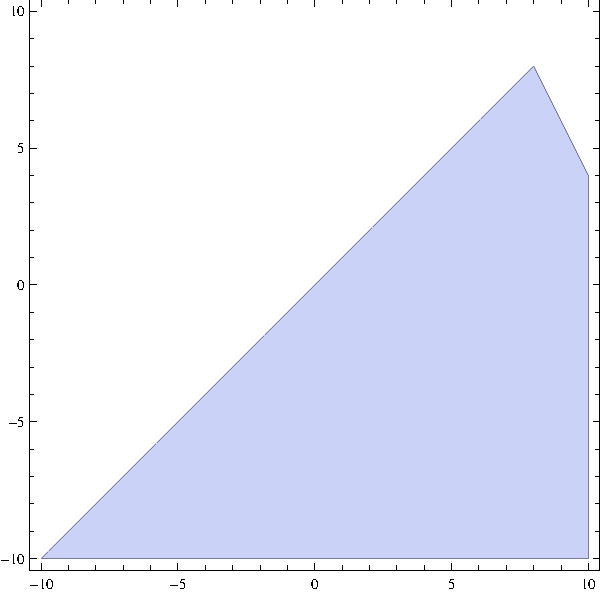
\includegraphics{graph2.pdf}
\newline\newline
The solution to a linear programming problem, as we learned in class, must exist on the extreme points in the simplex. The solution to this
problem is $x = 8, y=8 \rightarrow z = 16$ because it is the only extreme point on the simplex. We will prove this is indeed optimal in the next part
of the problem.
\newline
\newline
\textbf{2. Using the constraints of the program, prove that the solution you found in part $1$ is indeed optimal. }
\newline
\newline
As we learned in precept, the optimality criterion states that if a maximization primal and its dual have feasible solutions $w$ and $z$ respectively
such that $w = z$, then these are optimal to the primal and its dual respectively. Thus we show that the dual has a feasible solution that is equal to 
the primal at $x,y = 8 \rightarrow z = 16$. The corresponding dual to this programming problem is as follows:
\newline\newline
Minimize $w = 0y_1 + 10y_2 + 24y_3$ subject to
$$
\begin{cases}
-y_1 + y_2 + 2y_3 \geq 1 \\
y_1 + 0y_2 + y_3 \geq 1 
\end{cases}
$$
\newline
\newline
Letting $y_1 = 1/3, y_2 = 0, y_3 = 2/3$ satisfies these constraints, because  $-1/3 + 4/3 = 1 \geq 1$ and $1/3 + 2/3 = 1 \geq 1$, and yield
$0y_1 + 10y_2 + 24y_3 = 0 + 0 + 24 (2/3) = 16$. Further, this solution is optimal to the dual by the optimality criterion because it is equal to the optimal value of the 
primal.
\newline
\newline
Thus, having found a feasible solution in the maximization primal, $z=16$, and a solution in its dual, $w=16$, such that $w=z$, this solution
$x=8, y= 8, z=16$ is an optimal solution by the optimality criterion.
% End sol%

\pagebreak{}

\thispagestyle{empty}

\begin{tabular*}{1\textwidth}{@{\extracolsep{\fill}}lr}
\textbf{ID:} 03 & \textbf{Collaborator \#1:} Chen, Josh\tabularnewline
\textbf{Name:} Al-Naji, Nader & \textbf{Collaborator \#2:} Last Name, First Name\tabularnewline
\hline 
\end{tabular*}

\medskip{}


\begin{center}
\begin{Large}\textbf{Solution to HW 6, Problem 4}\end{Large}
\par\end{center}

\begin{center}
\begin{large}\textbf{COS 340 - Spring 2012}\end{large}
\par\end{center}

\bigskip{}


% Begin sol%
You are preparing for a bake with four basic ingredients at your disposal: $20$ lb of sugar,
$20$ lb of flour, $5$ lb of dried fruit, and $5$lb of chocolate chips. You are able to prepare any of the following recipes:
\begin{itemize}
\item Chocolate chip cookies: $1$lb flour, $.5$lb sugar, $.5$lb chocolate chips.
\item Fruit cake: $.5$lb flour, $1$lb sugar, $1$lb dried fruit.
\item Chocolate buns: $2.5$lb flour, $.5$lb sugar, $.25$lb chocolate chips.
\item Meringue cookies: $2$lb sugar.
\item Chocolate-fruit pizza: $2$lb flour, $1$lb sugar, $1$lb dried fruit, $1$lb chocolate chips.
\end{itemize}
You can prepare any fraction of a portion by using a proportionally reduced amount of ingredients. A portion of chocolate chip cookies sells for $\$10$,
a portion of fruit cake for $\$12$, a portion of buns for $\$14$, a portion of meringue sells for $\$7$ and a portion of the weird pizza sells for $\$2$.
\newline
\newline
\textbf{1. Formulate a linear program that would allow you to maximize the proceeds in the bake sale. Carefully state the variables, the constraints, and 
the objective. You don't need to solve the program.}
\newline
\newline
Let $r_1, ..., r_5$ denote the number of portions of each recipe listed in the order above that we decide to make respectively. If we choose to make $1$ portion of
$r_1$, for example, then we will require $1$lb of flour, $.5$lb sugar, $.5$lb of chocolate chips. If we choose to make twice that, then we will need double this amount, etc...
Thus, the amount of each ingredient that we will end up needing will be equal to the number of portions of each recipe that we decide to make multiplied by the amount
of that ingredient each recipe requires. Having noted this, along with the fact that the amount of each ingredient we use cannot exceed the above constraints and that the number
of portions of any given recipe cannot be negative, it should be clear that we have the following linear programming problem:
\newline\newline
Maximize $10r_1 + 12r_2 + 14r_3 + 7r_4 + 2r_5$ subject to:
\newline\newline
$$
\begin{cases}
.5r_1 + r_2 + .5r_3 + 2r_4 + r_5 \leq 20 \\
r_1 + .5r_2 + 2.5r_3 + 0r_4 + 2r_5 \leq 20 \\
0r_1 + r_2 + 0r_3 + 0r_4 + r_5 \leq 5 \\
.5r_1 + 0r_2 + .25r_3 + 0r_4 + r_5 \leq 5 \\
r_1, r_2, r_3, r_4, r_5 \geq 0
\end{cases}
$$
\newline\newline
\textbf{2. Now suppose that you are actually required to use up all the ingredients. How would you modify the program from part $1$ to address this 
constraint?}
\newline
\newline
All this does is cause the inequality signs above to become equality signs. Since we must use up all of our ingredients, the number of portions of each
recipe we construct must be chosen such that the amount of each ingredient we use is now equal to the amount we have. However, because we are not allowed
to actually have strict equality signs in a linear programming problem, we can substitute each strict equality with a $\geq$ and a $\leq$ inequality. Having noted this, it should be
clear that the modified problem looks as follows:
\newline
\newline
Maximize $10r_1 + 12r_2 + 14r_3 + 7r_4 + 2r_5$ subject to:
$$
\begin{cases}
.5r_1 + r_2 + .5r_3 + 2r_4 + r_5 \leq 20 \\
.5r_1 + r_2 + .5r_3 + 2r_4 + r_5 \geq 20 \\
r_1 + .5r_2 + 2.5r_3 + 0r_4 + 2r_5 \leq 20 \\
r_1 + .5r_2 + 2.5r_3 + 0r_4 + 2r_5 \geq 20 \\
0r_1 + r_2 + 0r_3 + 0r_4 + r_5 \leq 5 \\
0r_1 + r_2 + 0r_3 + 0r_4 + r_5 \geq 5 \\
.5r_1 + 0r_2 + .25r_3 + 0r_4 + r_5 \leq 5 \\
.5r_1 + 0r_2 + .25r_3 + 0r_4 + r_5 \geq 5 \\
r_1, r_2, r_3, r_4, r_5 \geq 0
\end{cases}
$$
\newline
\newline
And, turning all inequalities into $\leq$ without loss of generality we have:
\newline
\newline
Maximize $10r_1 + 12r_2 + 14r_3 + 7r_4 + 2r_5$ subject to:
$$
\begin{cases}
.5r_1 + r_2 + .5r_3 + 2r_4 + r_5 \leq 20 \\
-(.5r_1 + r_2 + .5r_3 + 2r_4 + r_5) \leq -20 \\
r_1 + .5r_2 + 2.5r_3 + 0r_4 + 2r_5 \leq 20 \\
-(r_1 + .5r_2 + 2.5r_3 + 0r_4 + 2r_5) \leq -20 \\
0r_1 + r_2 + 0r_3 + 0r_4 + r_5 \leq 5 \\
-(0r_1 + r_2 + 0r_3 + 0r_4 + r_5) \leq -5 \\
.5r_1 + 0r_2 + .25r_3 + 0r_4 + r_5 \leq 5 \\
-(.5r_1 + 0r_2 + .25r_3 + 0r_4 + r_5) \leq -5 \\
r_1, r_2, r_3, r_4, r_5 \geq 0
\end{cases}
$$
% End sol%

\pagebreak{}

\end{document}
